%
\hsection{Connect to the Database}%
\FloatBarrier%
%
%
We first need to connect from \libreofficeBase\ to the \postgresql\ \server\ and our \sqlil{factory}~\db.
We therefore open \libreofficeBase\ as discussed back in \cref{sec:installLibreOffice}.
In the opening screen, we choose \inQuotes{Connect to existing database} as shown in \cref{fig:factoryLibreOfficeBaseConnect01selectDatabase}, because that is what we want to do.
We need to select the \postgresql\ connector.
So we click on the driver drop-down box in \cref{fig:factoryLibreOfficeBaseConnect02connectToExisting}.
We select \postgresql\ as \db\ connection driver in \cref{fig:factoryLibreOfficeBaseConnect03postgres}.
Now that \postgresql\ is selected, we can click~\menu{Next} as shown in \cref{fig:factoryLibreOfficeBaseConnect04postgres}.

\begin{figure}%
\centering%
%
\subfloat[][%
In the \libreofficeBase\ opening screen, we choose \inQuotes{Connect to existing database.}%
\label{fig:factoryLibreOfficeBaseConnect01selectDatabase}%
]{\tightbox{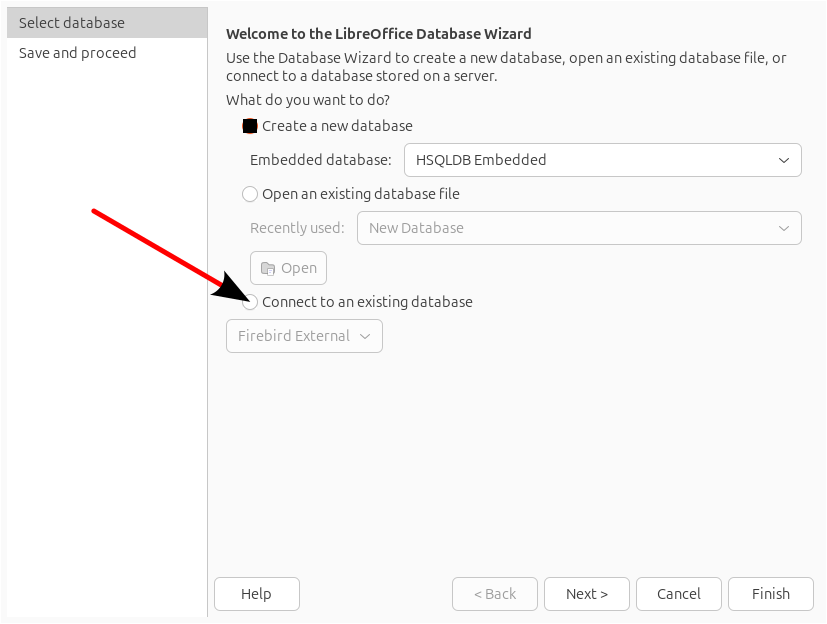
\includegraphics[width=0.49\linewidth]{\currentDir/factoryLibreOfficeBaseConnect01selectDatabase}}}%
%
\floatSep%
%
\subfloat[][%
We then click on the \db\ driver drop-down box.%
\label{fig:factoryLibreOfficeBaseConnect02connectToExisting}%
]{\tightbox{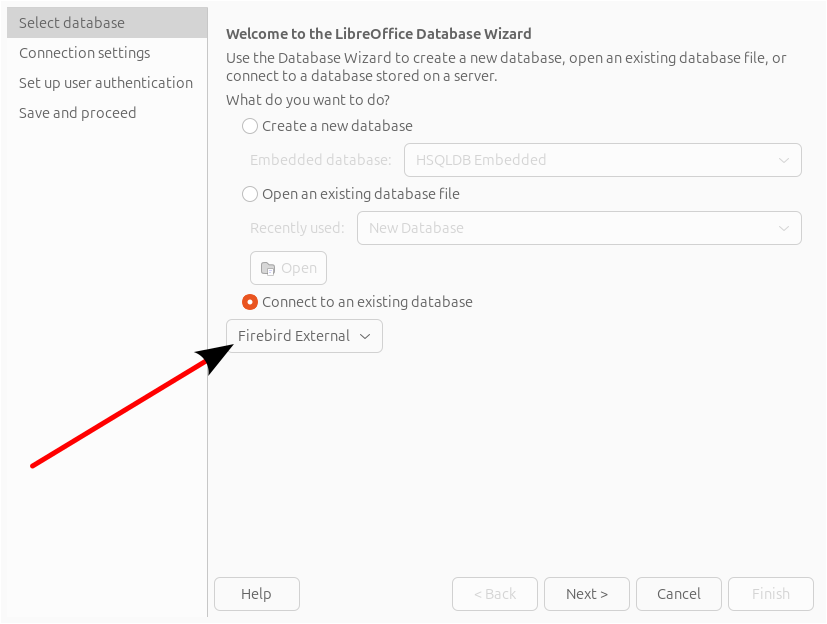
\includegraphics[width=0.49\linewidth]{\currentDir/factoryLibreOfficeBaseConnect02connectToExisting}}}%
%
\floatRowSep%
%
\subfloat[][%
We select \postgresql\ as \db\ driver.%
\label{fig:factoryLibreOfficeBaseConnect03postgres}%
]{\tightbox{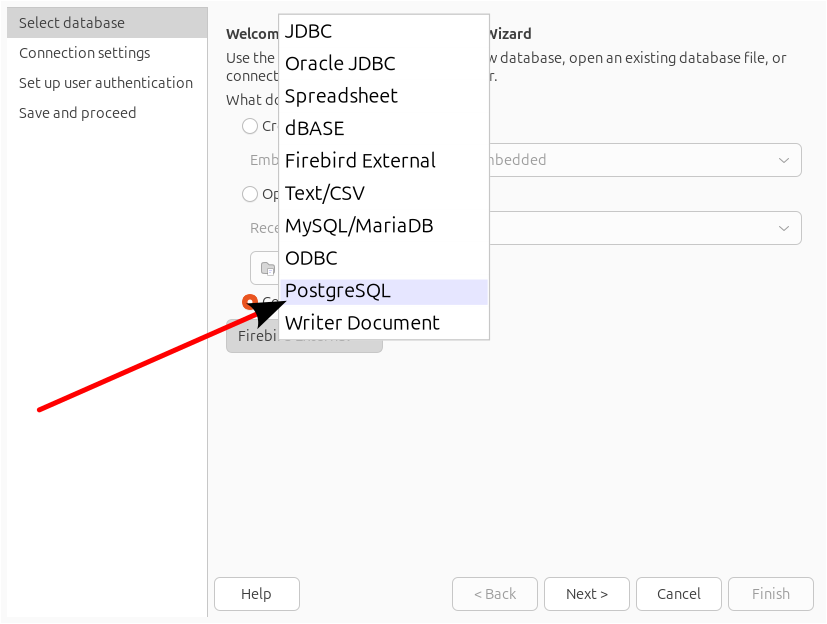
\includegraphics[width=0.49\linewidth]{\currentDir/factoryLibreOfficeBaseConnect03postgres}}}%
%
\floatSep%
%
\subfloat[][%
Once \postgresql\ is selected, we can click \menu{Next}.%
\label{fig:factoryLibreOfficeBaseConnect04postgres}%
]{\tightbox{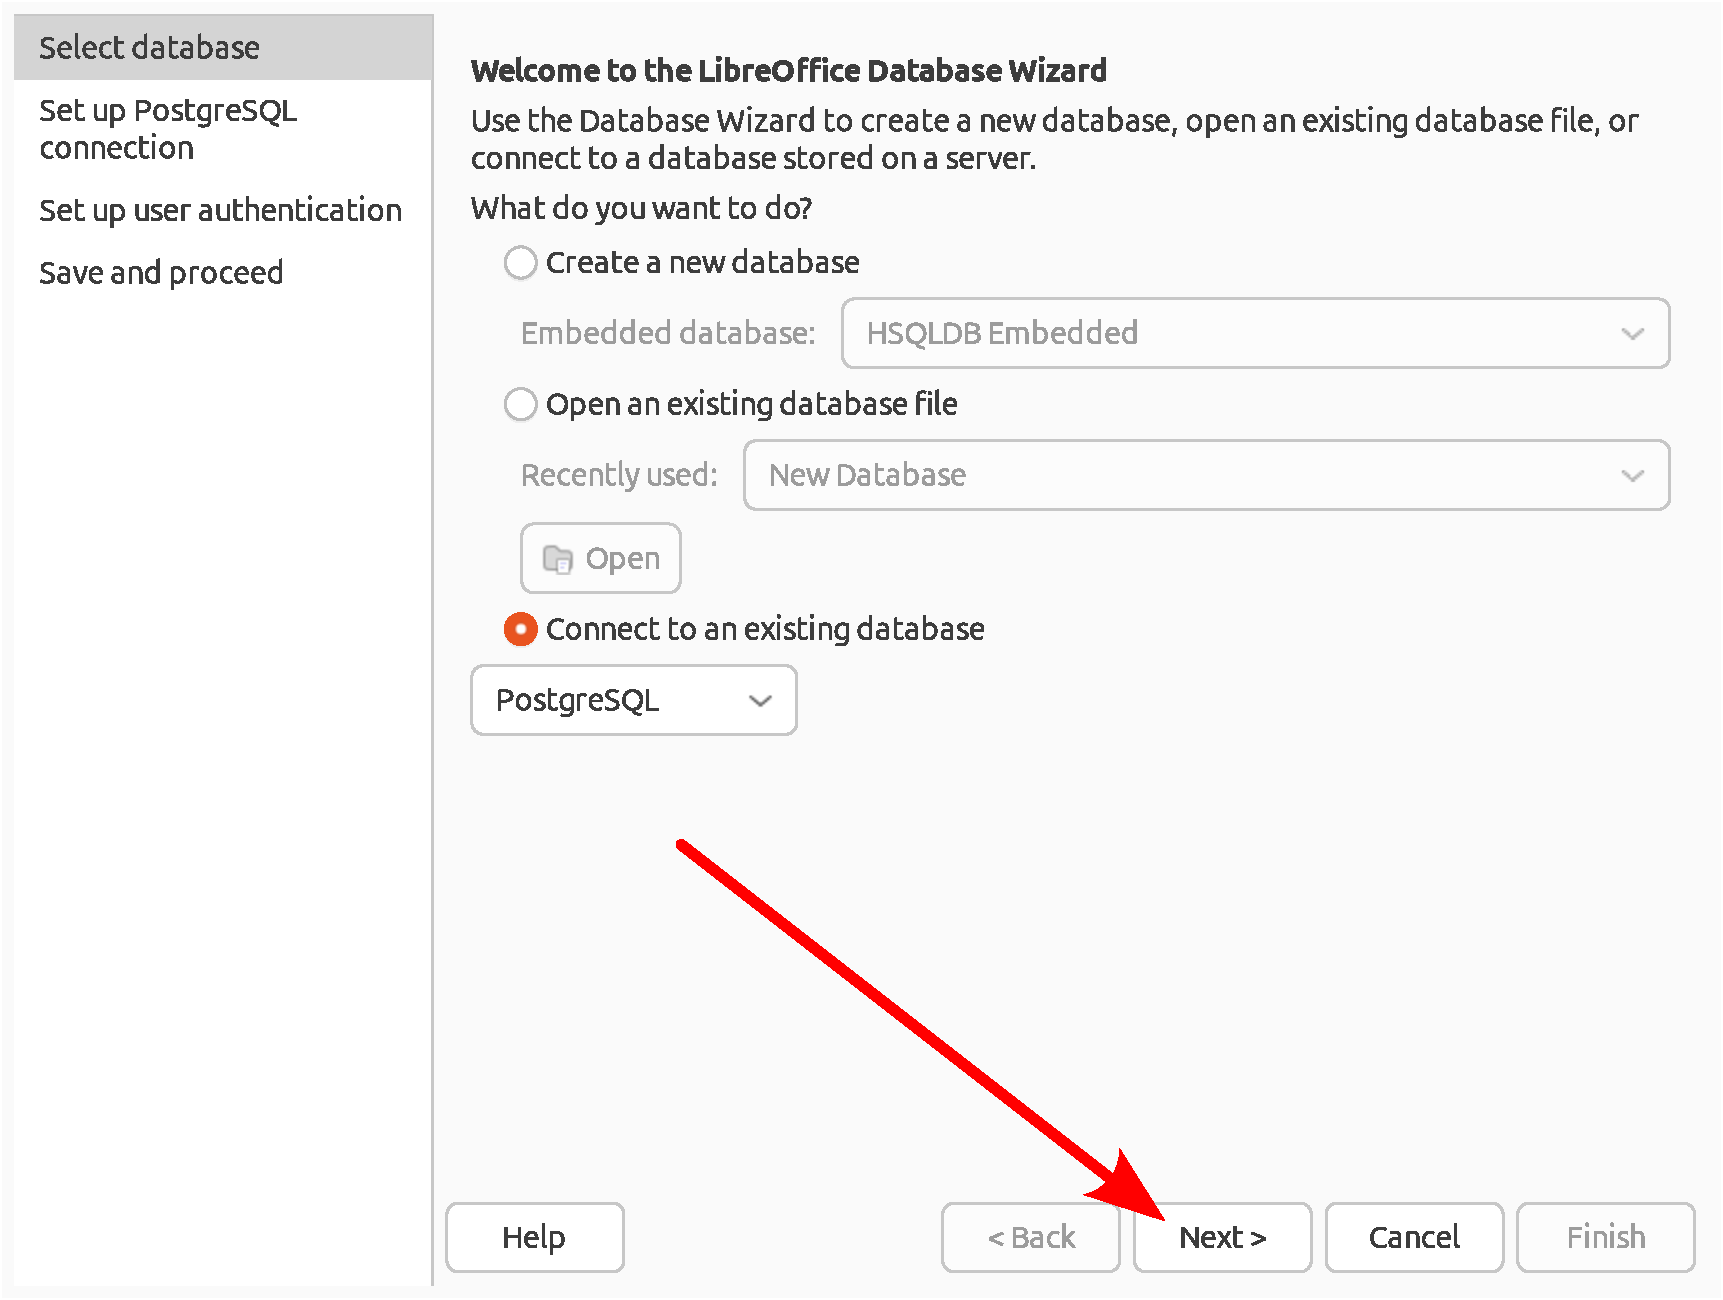
\includegraphics[width=0.49\linewidth]{\currentDir/factoryLibreOfficeBaseConnect04postgres}}}%
%
\floatRowSep%
%
\subfloat[][%
We enter \textil{factory} as \db\ name, \localhost\ as \server, 5321~as \pgls{port}, and then click \menu{Next}.%
\label{fig:factoryLibreOfficeBaseConnect05connection}%
]{\tightbox{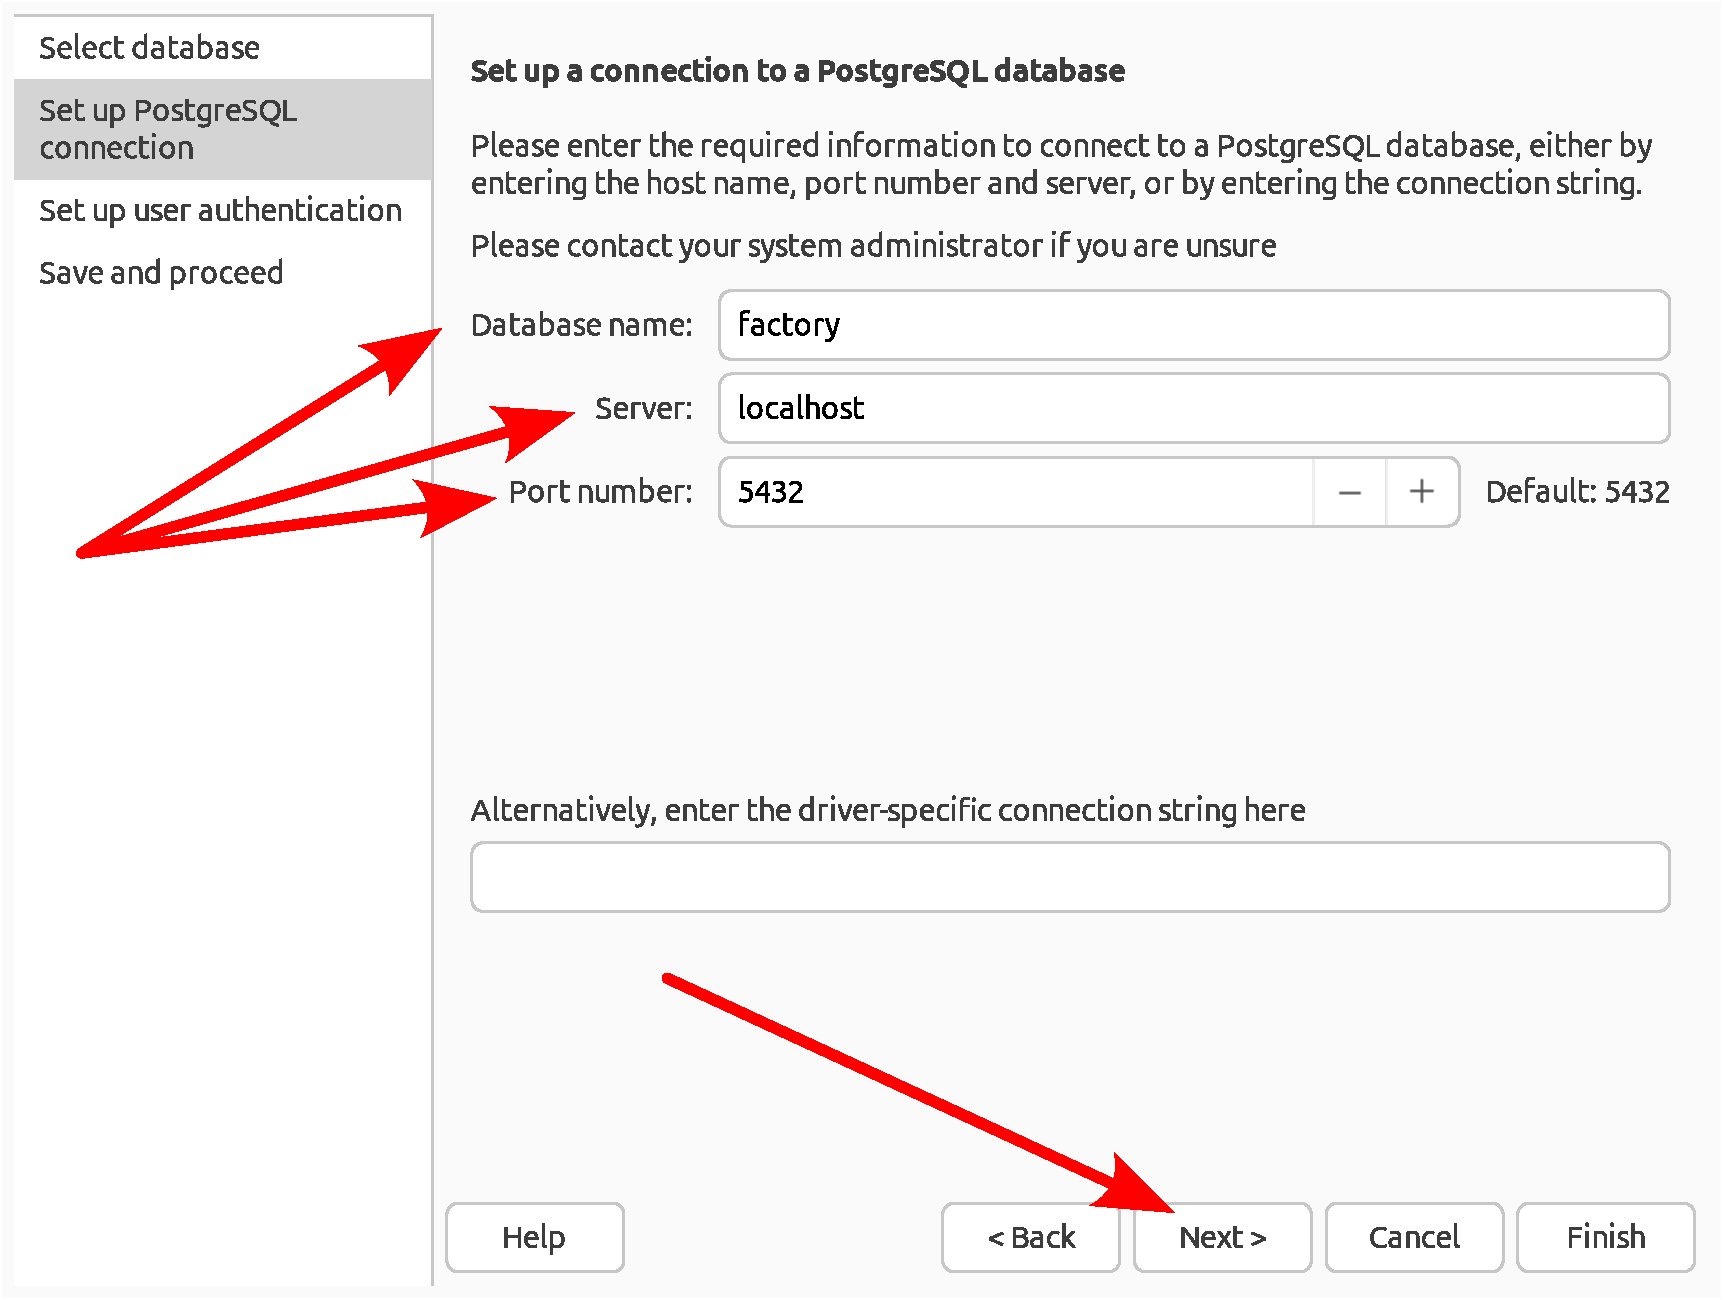
\includegraphics[width=0.49\linewidth]{\currentDir/factoryLibreOfficeBaseConnect05connection}}}%
%
\floatSep%
%
\subfloat[][%
As user name we enter \textil{boss} and select \menu{Password required}. %
Then we click \menu{Test Connection}.%
\label{fig:factoryLibreOfficeBaseConnect06authentication}%
]{\tightbox{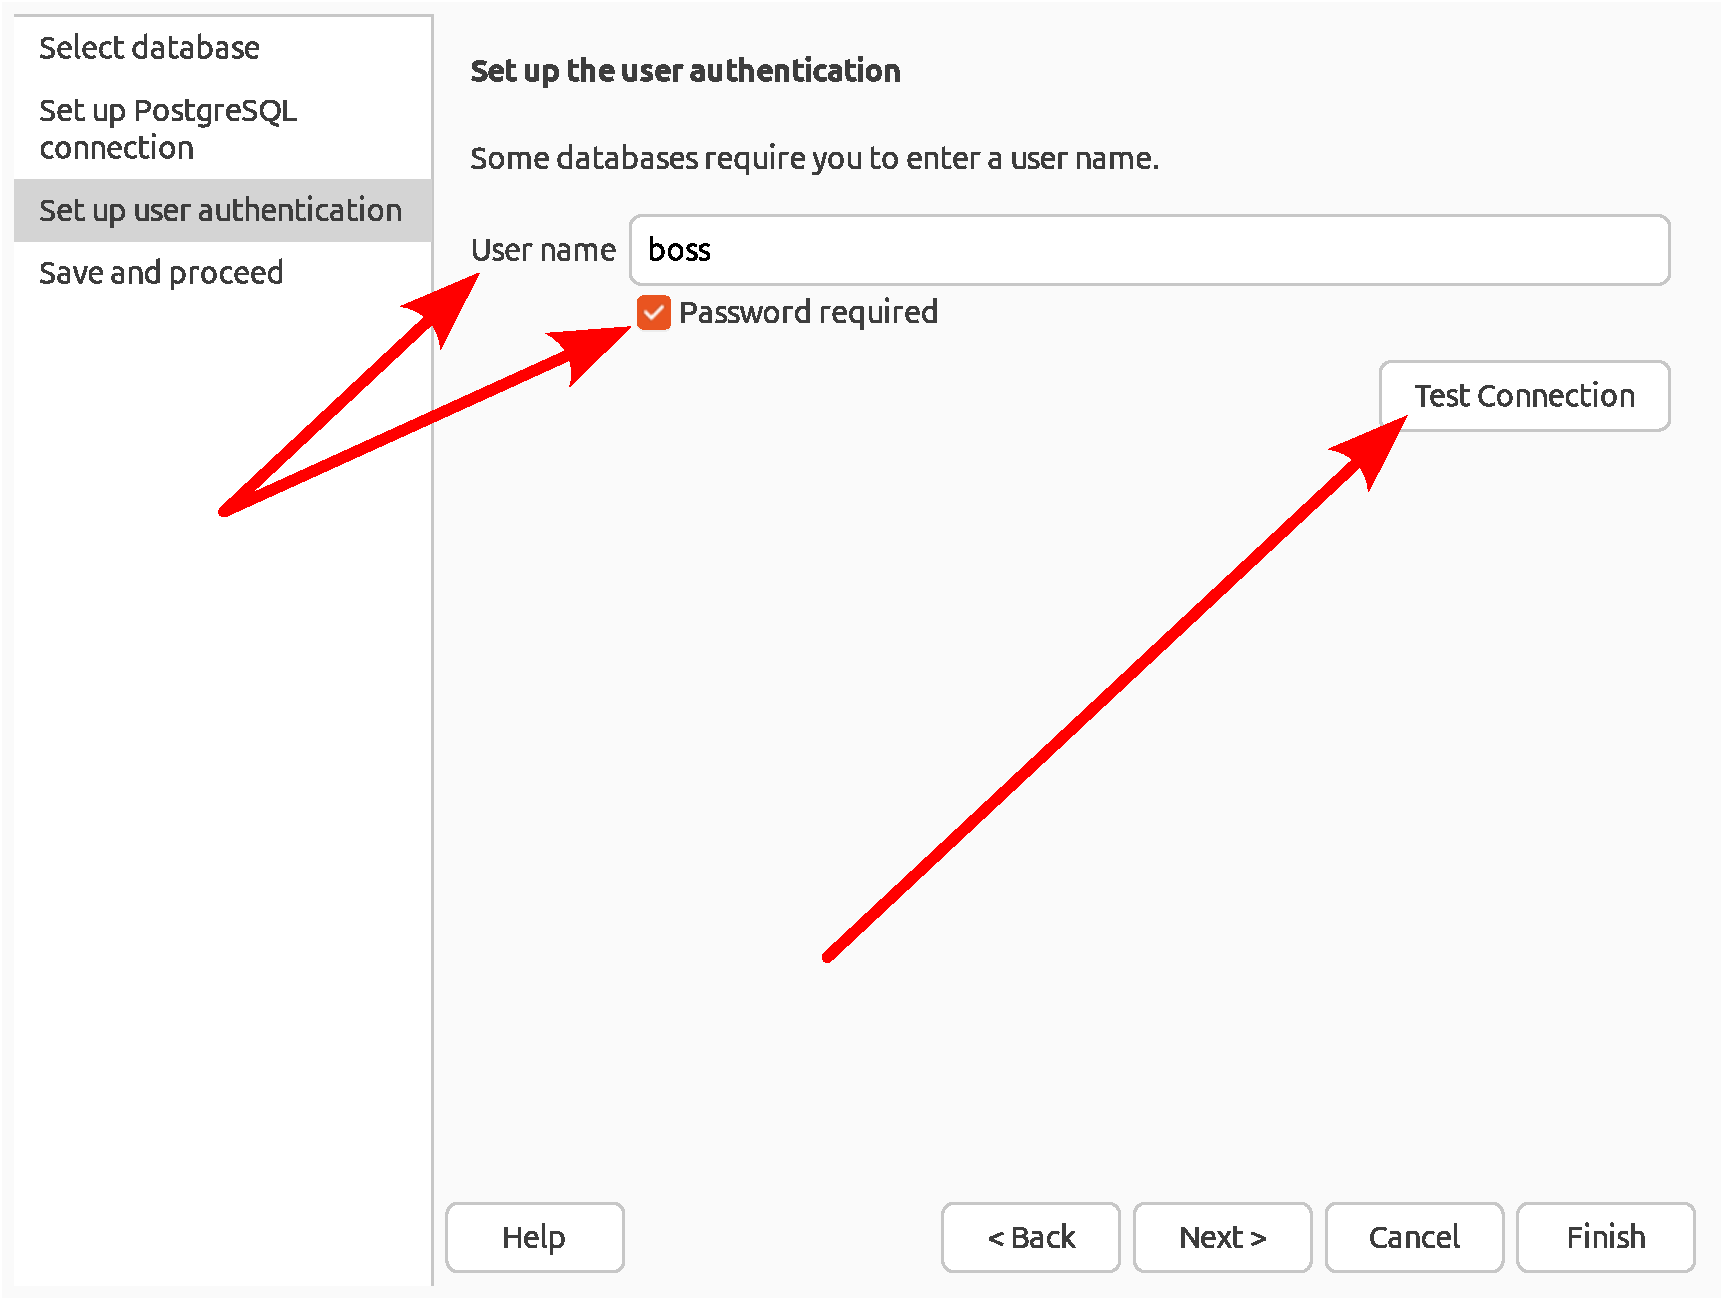
\includegraphics[width=0.49\linewidth]{\currentDir/factoryLibreOfficeBaseConnect06authentication}}}%
%
\caption{Connecting to our example \emph{factory} \db\ using \libreofficeBase.}%
\label{fig:factoryLibreOfficeBaseConnectA}%
%
\end{figure}%
%
%
\begin{figure}%
\ContinuedFloat%
\centering%
%
\subfloat[][%
In the authentication window, we enter the password \textil{superboss123} and click~\menu{OK}.%
\label{fig:factoryLibreOfficeBaseConnect07test}%
]{\tightbox{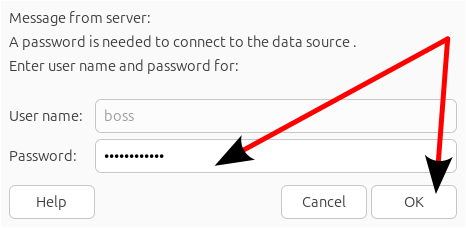
\includegraphics[width=0.49\linewidth]{\currentDir/factoryLibreOfficeBaseConnect07test}}}%
%
\floatSep%
%
\subfloat[][%
We get notified that the connection succeeded. We click~\menu{OK}.%
\label{fig:factoryLibreOfficeBaseConnect08testSuccess}%
]{\tightbox{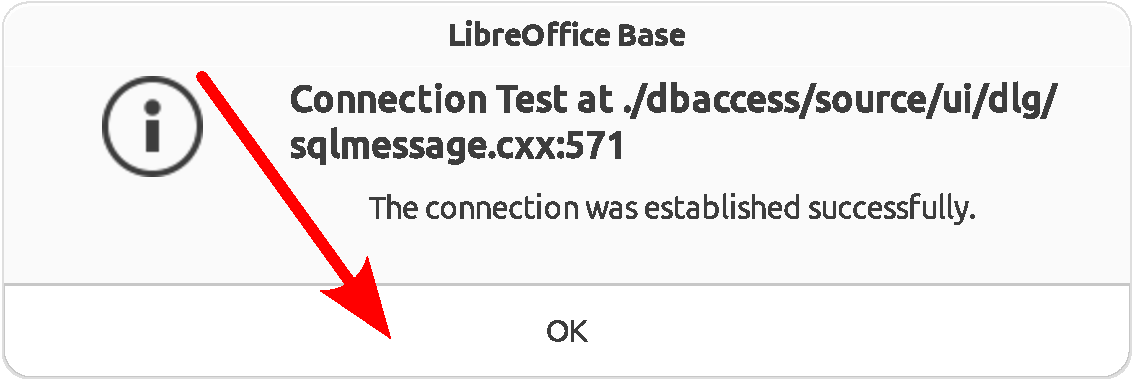
\includegraphics[width=0.49\linewidth]{\currentDir/factoryLibreOfficeBaseConnect08testSuccess}}}%
%
\floatRowSep%
%
\subfloat[][%
We now can click \menu{Next} in the authentication menu.%
\label{fig:factoryLibreOfficeBaseConnect09authenticationNext}%
]{\tightbox{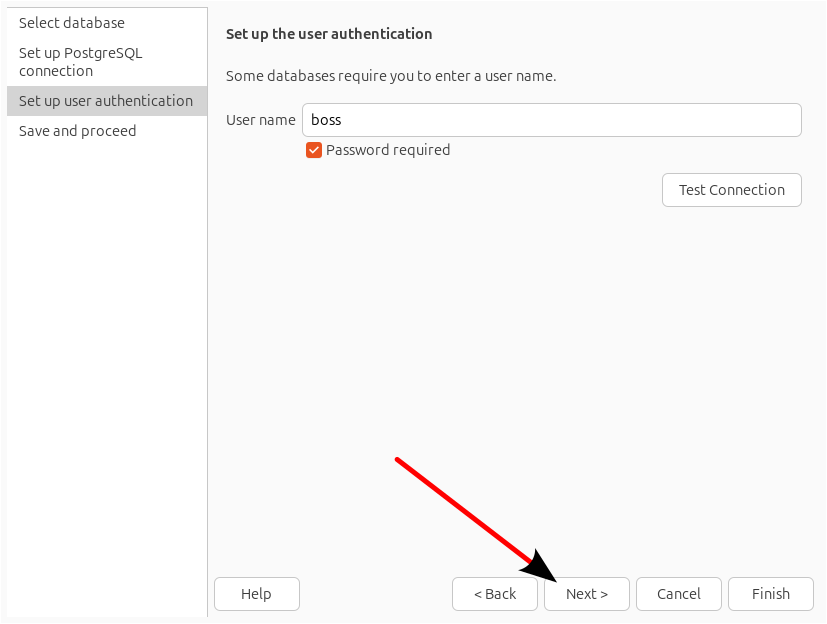
\includegraphics[width=0.49\linewidth]{\currentDir/factoryLibreOfficeBaseConnect09authenticationNext}}}%
%
\floatSep%
%
\subfloat[][%
We do not want to register the \db, we want to open it for editing, and click \menu{Finish}.%
\label{fig:factoryLibreOfficeBaseConnect10notRegister}%
]{\tightbox{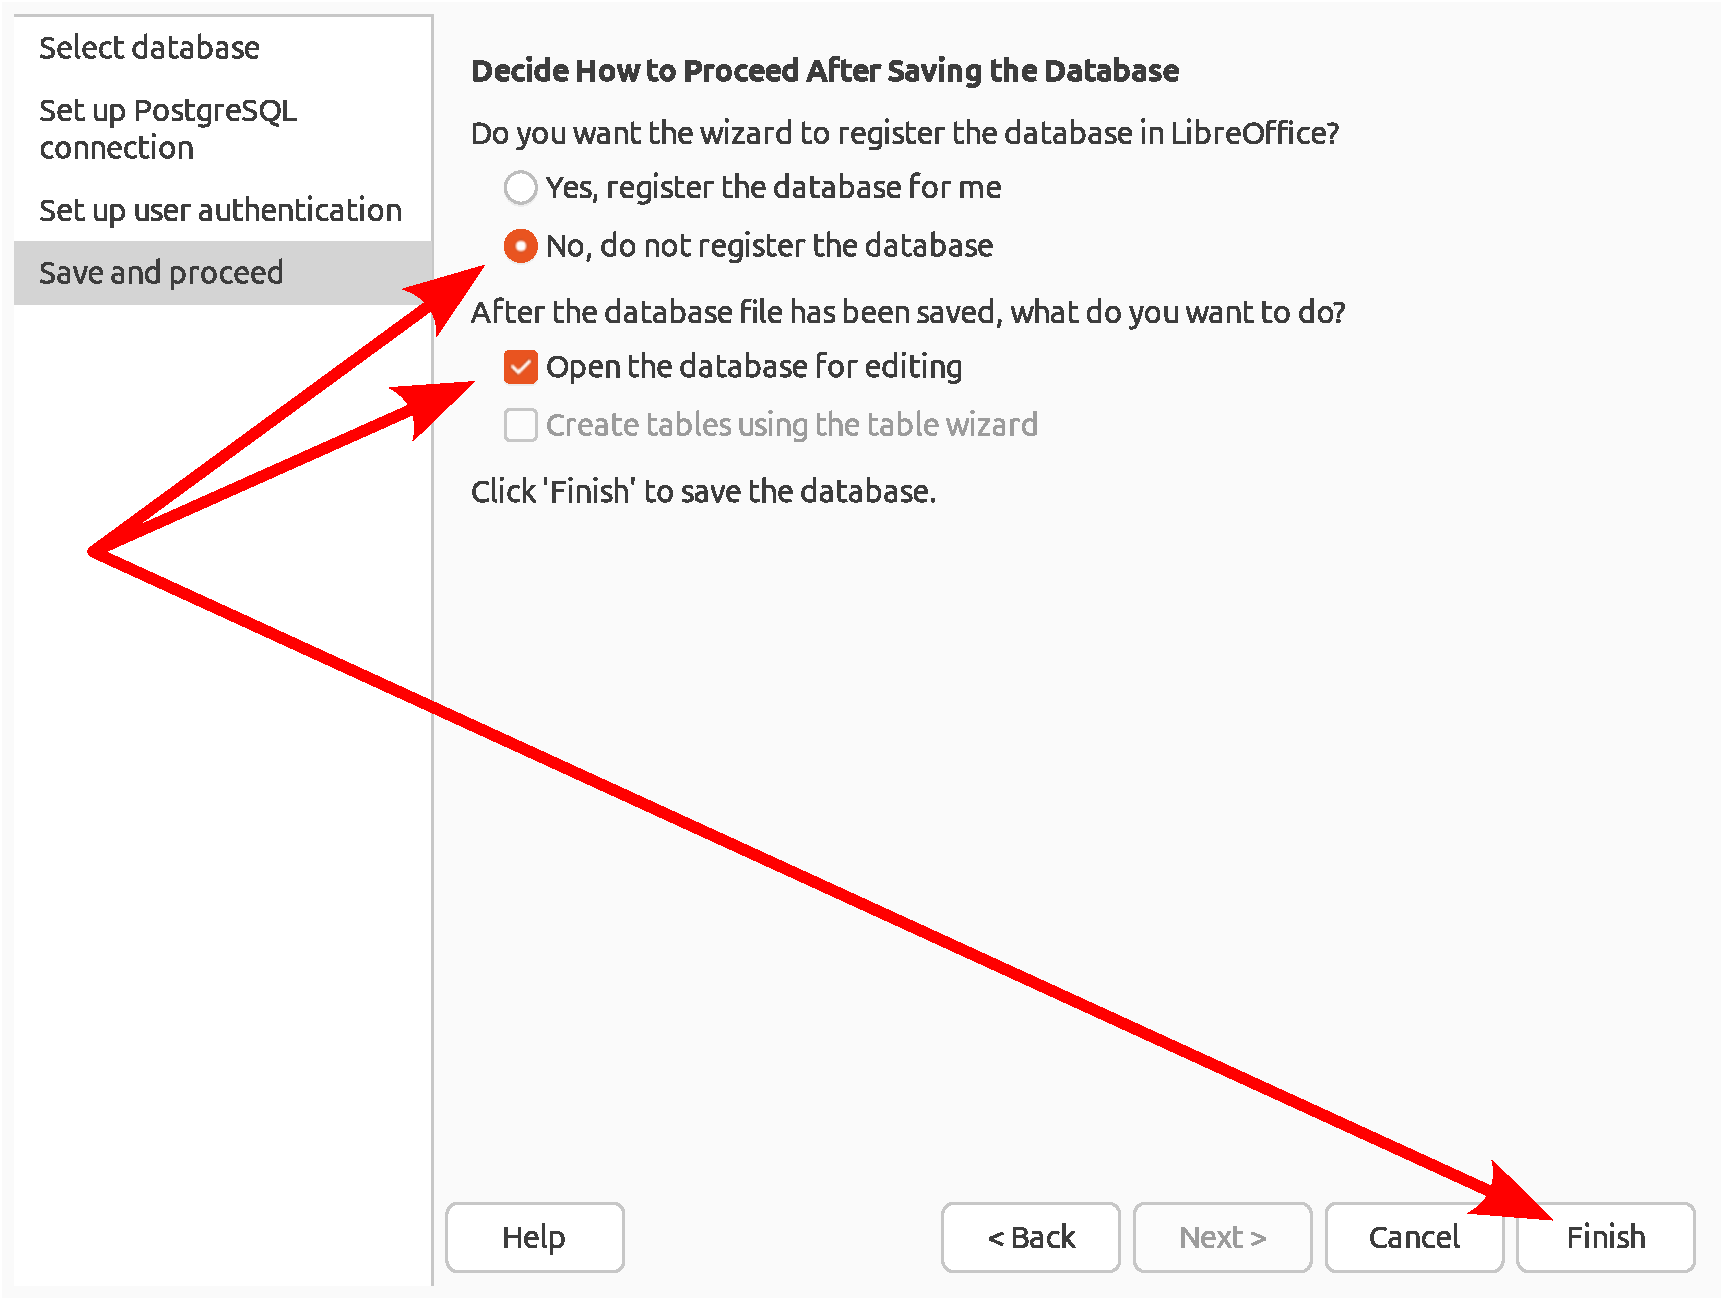
\includegraphics[width=0.49\linewidth]{\currentDir/factoryLibreOfficeBaseConnect10notRegister}}}%
%
\floatRowSep%
%
\subfloat[][%
We now save the \libreofficeBase\ document to a suitable file.%
\label{fig:factoryLibreOfficeBaseConnect11save}%
]{\tightbox{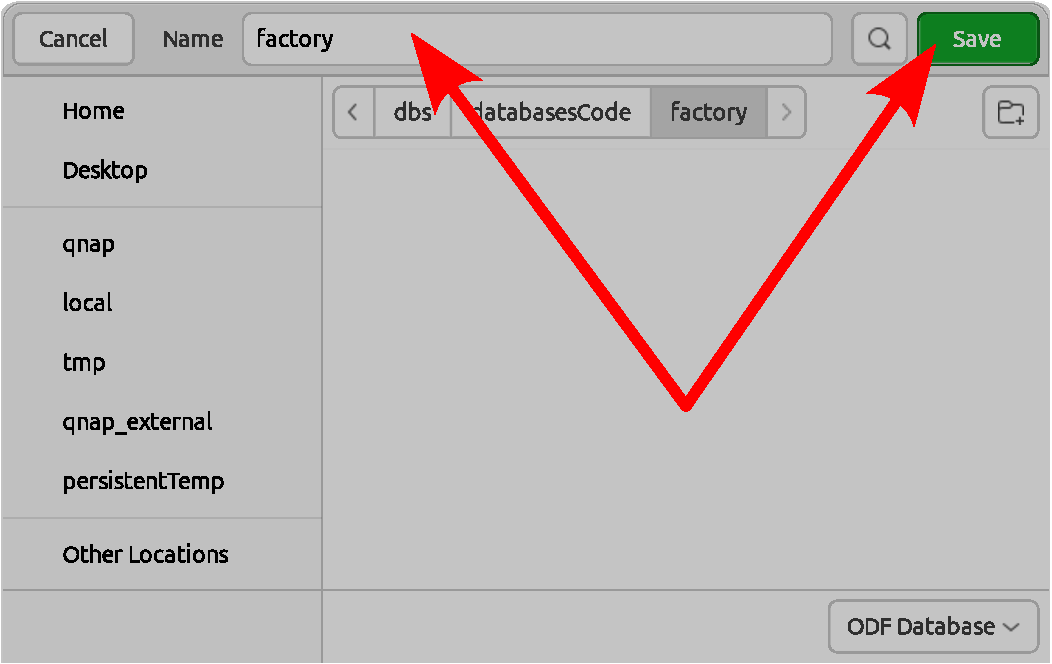
\includegraphics[width=0.49\linewidth]{\currentDir/factoryLibreOfficeBaseConnect11save}}}%
%
\floatRowSep%
%
\subfloat[][%
In the newly opened screen, we go into the \menu{Tables} pane and scroll down.%
\label{fig:factoryLibreOfficeBaseConnect12openingScreen}%
]{\tightbox{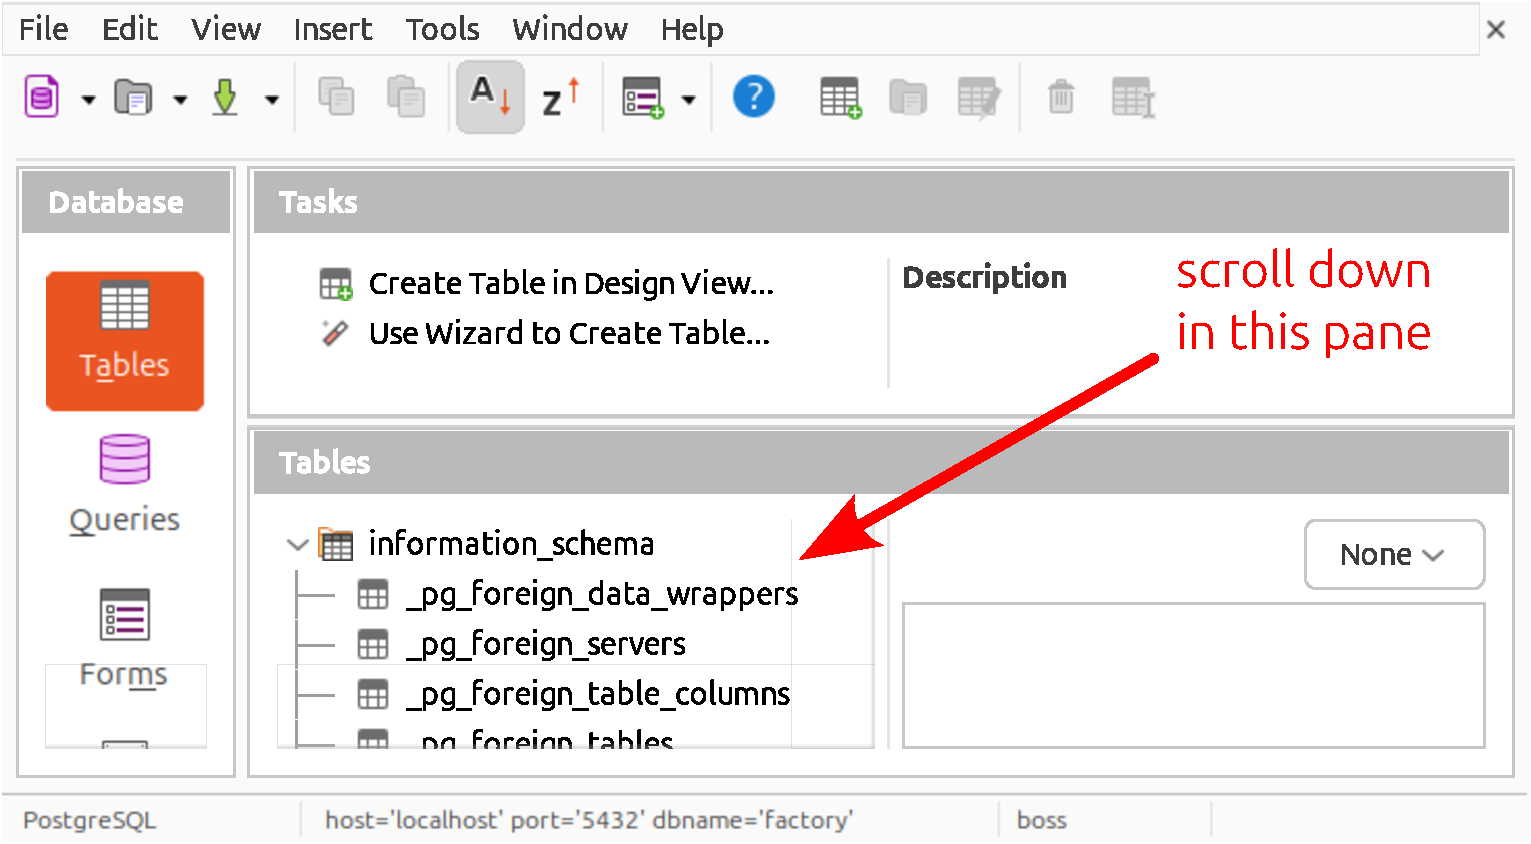
\includegraphics[width=0.49\linewidth]{\currentDir/factoryLibreOfficeBaseConnect12openingScreen}}}%
%
\floatSep%
%
\subfloat[][%
If we scroll down to the \menu{public} node, we can find our three tables and the view~\sqlil{sale}.%
\label{fig:factoryLibreOfficeBaseConnect13publicTables}%
]{\tightbox{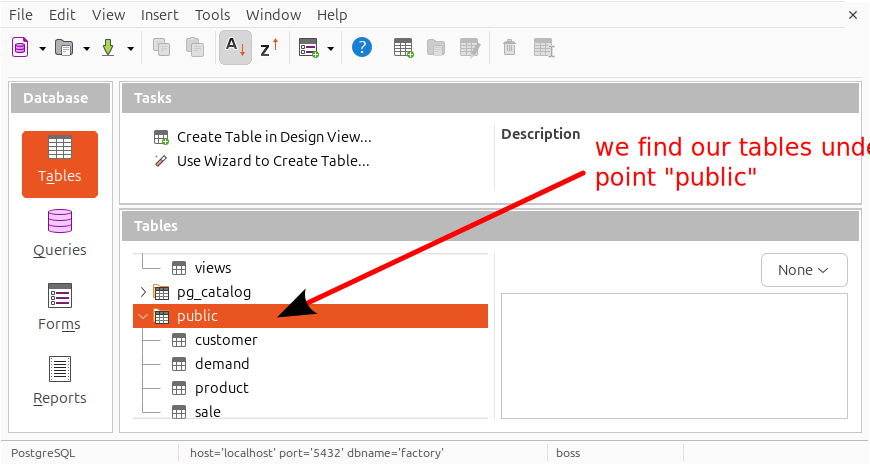
\includegraphics[width=0.49\linewidth]{\currentDir/factoryLibreOfficeBaseConnect13publicTables}}}%
%
\caption{Connecting to our example \emph{factory} \db\ using \libreofficeBase.}%
\label{fig:factoryLibreOfficeBaseConnectB}%
%
\end{figure}

In the next screen, we need to enter the information about the \dbms\ and \db\ we want to connect to.
The name of the \db\ is \textil{factory}.
As \server, we select \localhost, because the \dbms\ is running on our local computer.
Of course, if the \dbms\ was running on another computer, we could enter its IP~address here.
As \pgls{port}, we select the standard \postgresql\ \pgls{port}~5321.
Then we click \menu{Next} in \cref{fig:factoryLibreOfficeBaseConnect05connection}.

In the following screen, we enter the authentication information.
This is how \libreofficeBase\ will log into the \dbms.
We can enter the user name, which is \textil{boss}.
We had set the password \textil{superboss123} for this user, but we cannot enter it here.
It has to be entered explicitly everytime we open this connection.
This is probably in order to avoid storing sensible data, like a password, in the \libreofficeBase\ document.
This way, credentials cannot get lost or accidentally published when sharing the document with other users.
Either way, for this reason we need to select \menu{Password required}, because, yes, we have to authenticate the user \textil{boss} via password.
In \cref{fig:factoryLibreOfficeBaseConnect06authentication}, we then click \menu{Test Connection}.

In the authentication window that pops up in \cref{fig:factoryLibreOfficeBaseConnect07test}, we enter the password \textil{superboss123} and click~\menu{OK}.
As you can see in \cref{fig:factoryLibreOfficeBaseConnect08testSuccess}, the connection succeeded.
We close this dialog by clicking~\menu{OK}.

Back in the authentication screen in \cref{fig:factoryLibreOfficeBaseConnect09authenticationNext}, we can now click \menu{Next} in the authentication menu.
That takes us to the final screen of the \db\ document creation dialog.
We choose that we do not want to register the \db.
We choose that we want to open it for editing.
Finally, we click \menu{Finish} in \cref{fig:factoryLibreOfficeBaseConnect10notRegister}.

We now have to save the \libreofficeBase\ document to a suitable file.
The file type is \textil{odb}, which is basically a zip-compressed collection of \pgls{XML}~documents.
Be that as it be, we choose \textil{factory.odb} as file name in \cref{fig:factoryLibreOfficeBaseConnect11save}.

Finally, the \db\ \pgls{GUI} opens up.
We can see lots of stuff.
First, let us look for the \db\ objects we already have created.
In the newly opened screen, we go into the \menu{Tables} pane and scroll down in \cref{fig:factoryLibreOfficeBaseConnect12openingScreen}.
If we scroll down to the \menu{public} node, we can find our three tables and the view~\sqlil{sale}, as shown in \cref{fig:factoryLibreOfficeBaseConnect13publicTables}.
We successfully have connected to our example \db\ and can now work with it from the \libreofficeBase\ \pgls{GUI}.%
%
\FloatBarrier%
\endhsection%
%
